\section{The Composite Stellar Population Library}
\label{chap1:sec:SFHs}

In order to generate the eigenvectors composing the principal component space, we first generate training data using theoretical models of SFHs. Training spectra are generated by passing a piecewise-continuous star formation history (according to a randomized prescription described below) through a stellar population synthesis library, after assuming a stellar initial mass function (IMF), a set of isochrones, and a stellar library. In this case, the \texttt{fortran} code \texttt{Flexible Stellar Population Synthesis} (\texttt{FSPS}) \citep{fsps_1, fsps_2, fsps_3} and its \texttt{python} bindings \citep{pyfsps_DFM} were used. Padova 2008 \citep{marigo_08} isochrones were adopted. 

The unpublished C3K library of theoretical stellar spectra \citetext{Conroy, in prep.} was used for the population synthesis: the library is based on the Kurucz frameworks (routines and line lists)edit2{, and} the native resolution is $R=10,000$ from 1500$\mbox{\AA}$ to 1.1${\rm \mu}$m. Though most similar studies employ empirical stellar libraries \citep[e.g. MILES or E-MILES:][]{vazdekis10, vazdekis_16_e-miles}, there is at this time no widely-used library which closely matches the MaNGA wavelength range and resolution while covering the full stellar age and metallicity range expected in MaNGA. The latest E-MILES stellar population models, for instance, match MaNGA resolution and wavelength range, but have few stars younger than 0.1 Gyr at solar metallicity and above \citep[see][Figures 5 and 6]{vazdekis_16_e-miles}.

\subsection{SFHs and stellar population properties}

In order for the PCA model to emulate observed galaxy spectra, it must first be ``trained" to recognize what they can look like (that is, PCA ``learns" which wavelengths tend to vary together, and how strongly). By generating a plausible library of SFHs and their associated spectra, we provide the initial guidelines informing how real, observed spectra are fit. Since any fit to an observed spectrum must fall within the circumscribed domain of the training data, it is important to make that training data permissive enough to encompass physical reality. With too restrictive a training set, fits would suffer from additional systematic bias. As such, our SFH template parameters are intended to have weakly informative priors \citep{simpson_rue_14_priors, gelman_hennig_15} which encompass the areas of parameter space that are physically allowable and in line with previous studies (to this point, see the below description of the mass weighted mean stellar age distribution, Figure \ref{fig:mwa_dist}), while allowing only a relatively small proportion of more complex models (e.g., those involving bursts or a transition in SFH behavior).

Distributions of most parameters provided to \texttt{FSPS}, selected resulting stellar absorption indices, and other derived parameters of interest are respectively shown in Figures \ref{fig:prior_inputparams}, \ref{fig:prior_specinds}, and \ref{fig:prior_otherderived}, in addition to the full-text descriptions provided below.

\begin{figure*}
    \centering
    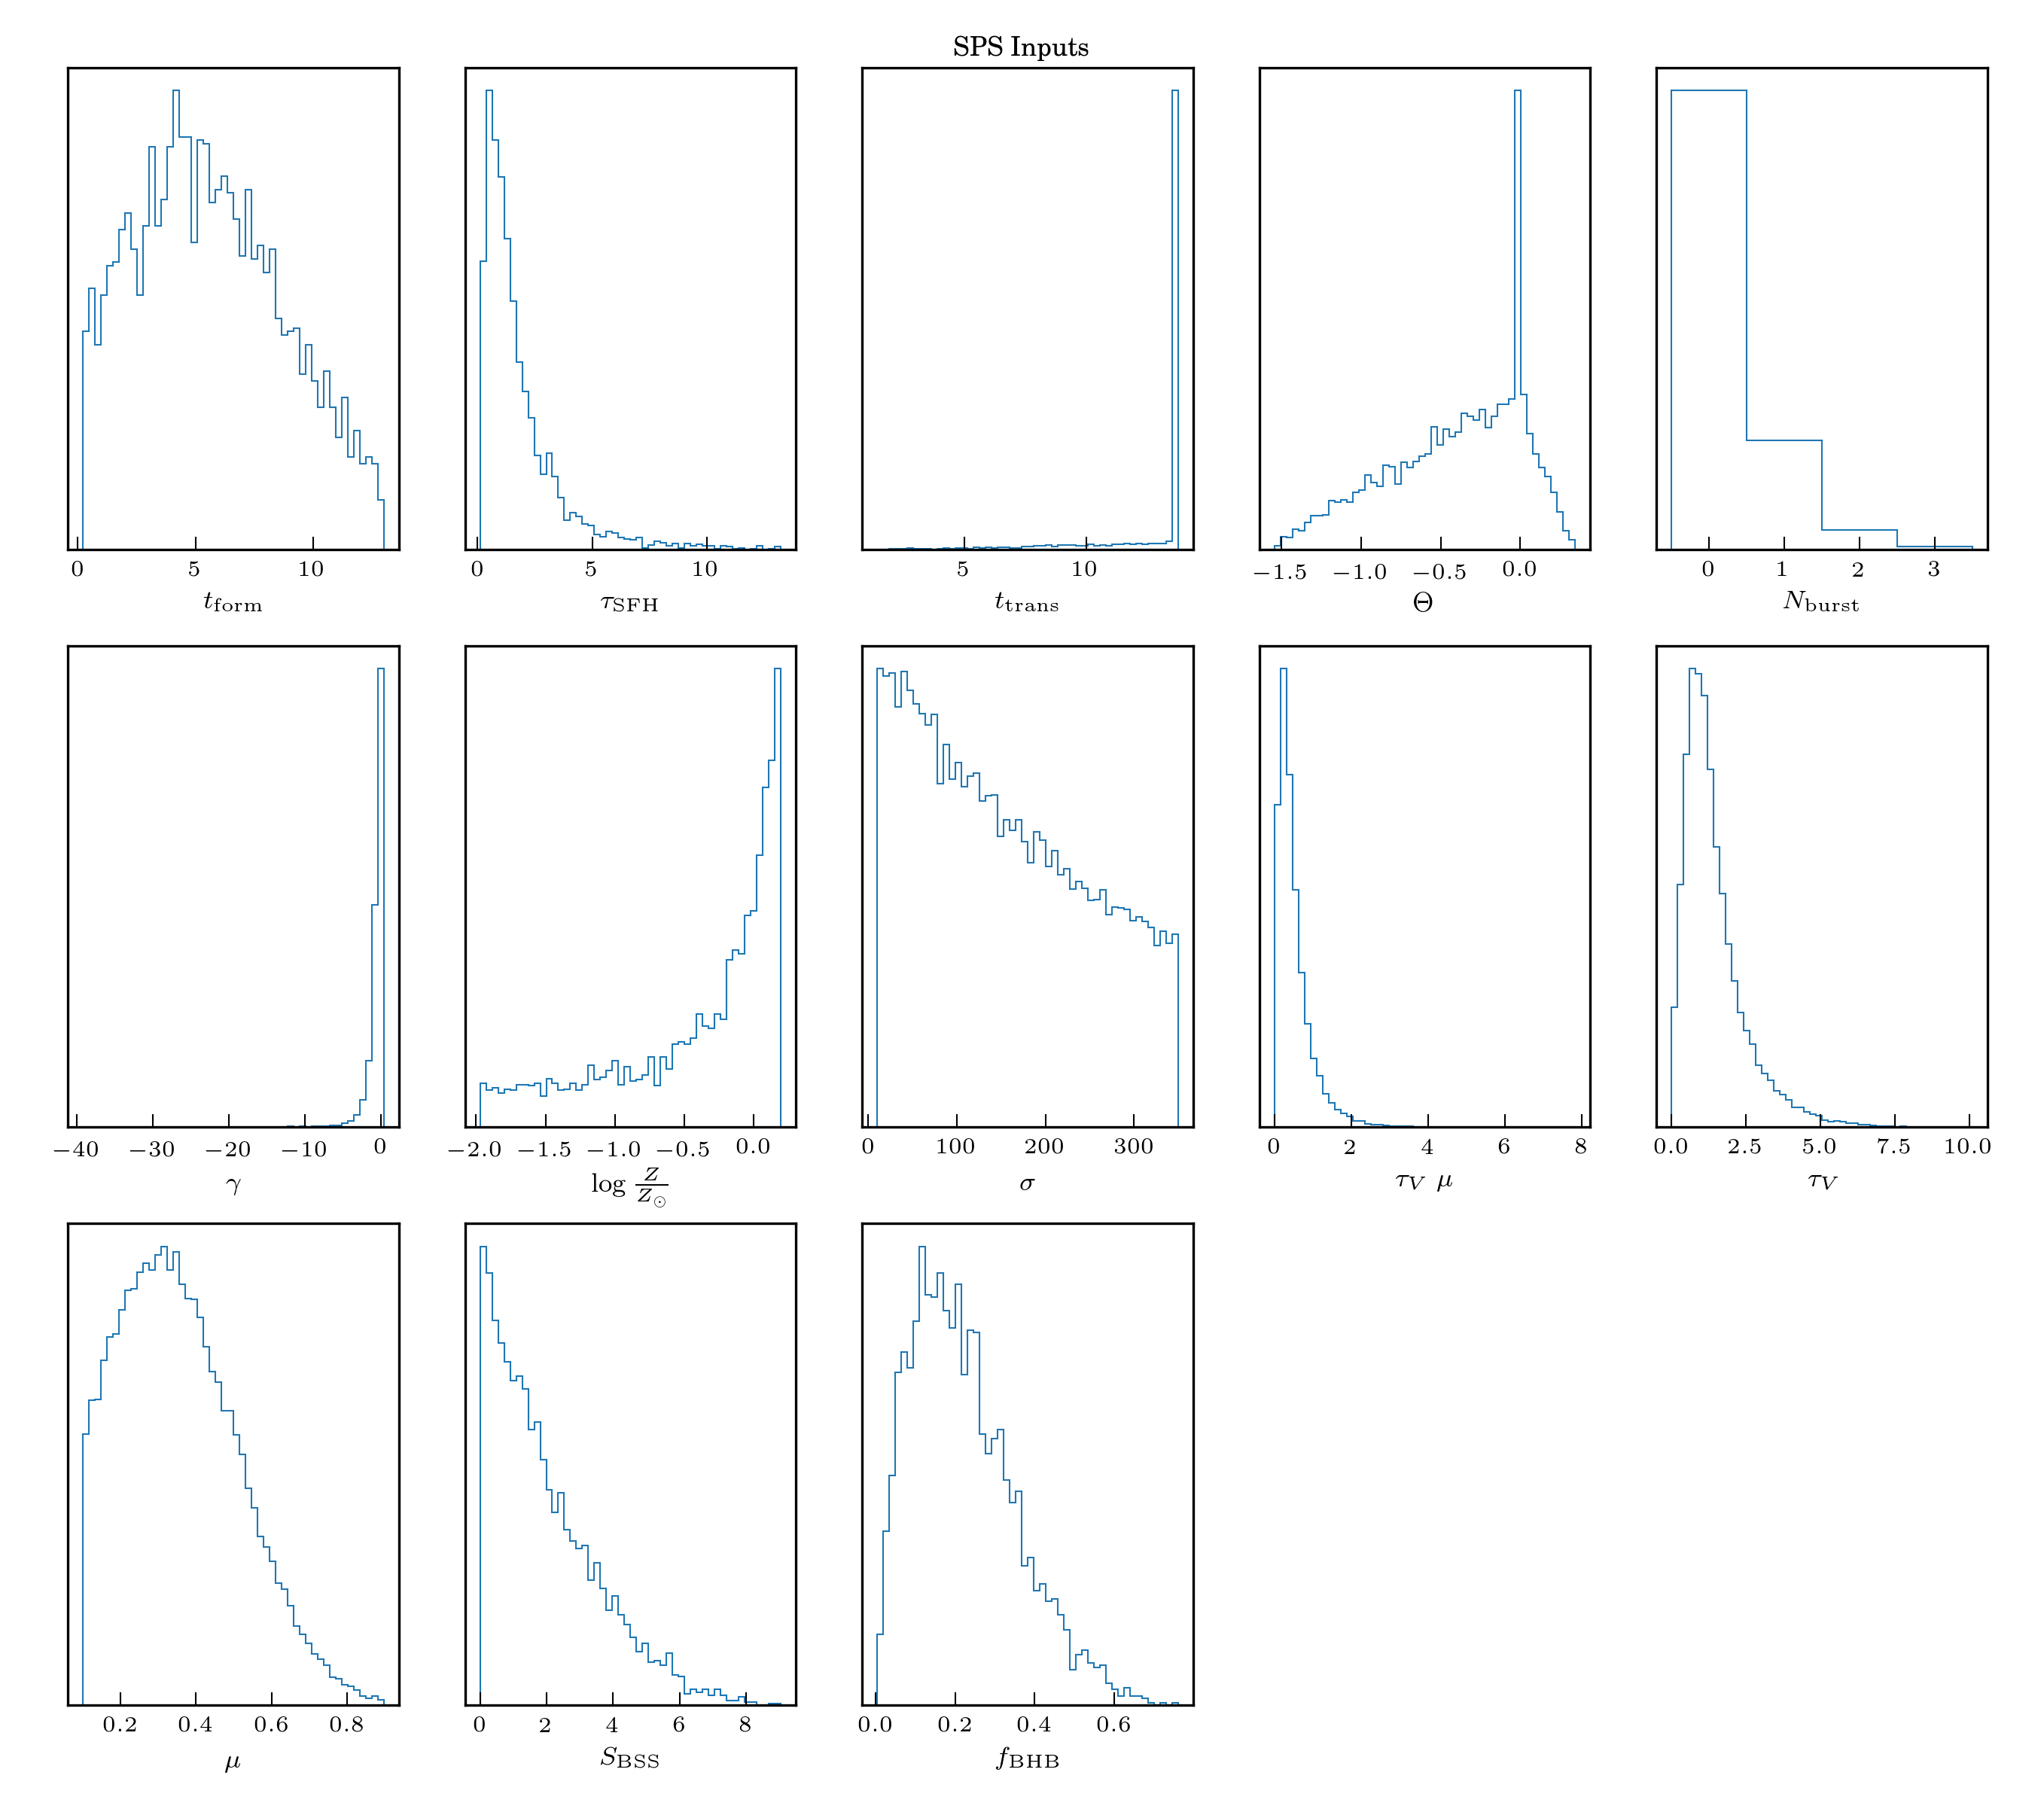
\includegraphics[width=\textwidth]{prior_inputparams}
    \caption[Distributions of stellar population synthesis inputs]{\fixspacing The distributions of the inputs provided to \texttt{FSPS} described in more detail in Section \ref{chap1:sec:SPS_params}, left to right and top to bottom: formation time, e-folding time, transition time, transition strength, transition slope, number of bursts, stellar metallicity, stellar velocity dispersion, attenuation, specific frequency of blue straggler stars, and fraction of blue horizontal branch stars. There is no covariance between these parameters.}
    \label{fig:prior_inputparams}
\end{figure*}

\begin{figure*}
    \centering
    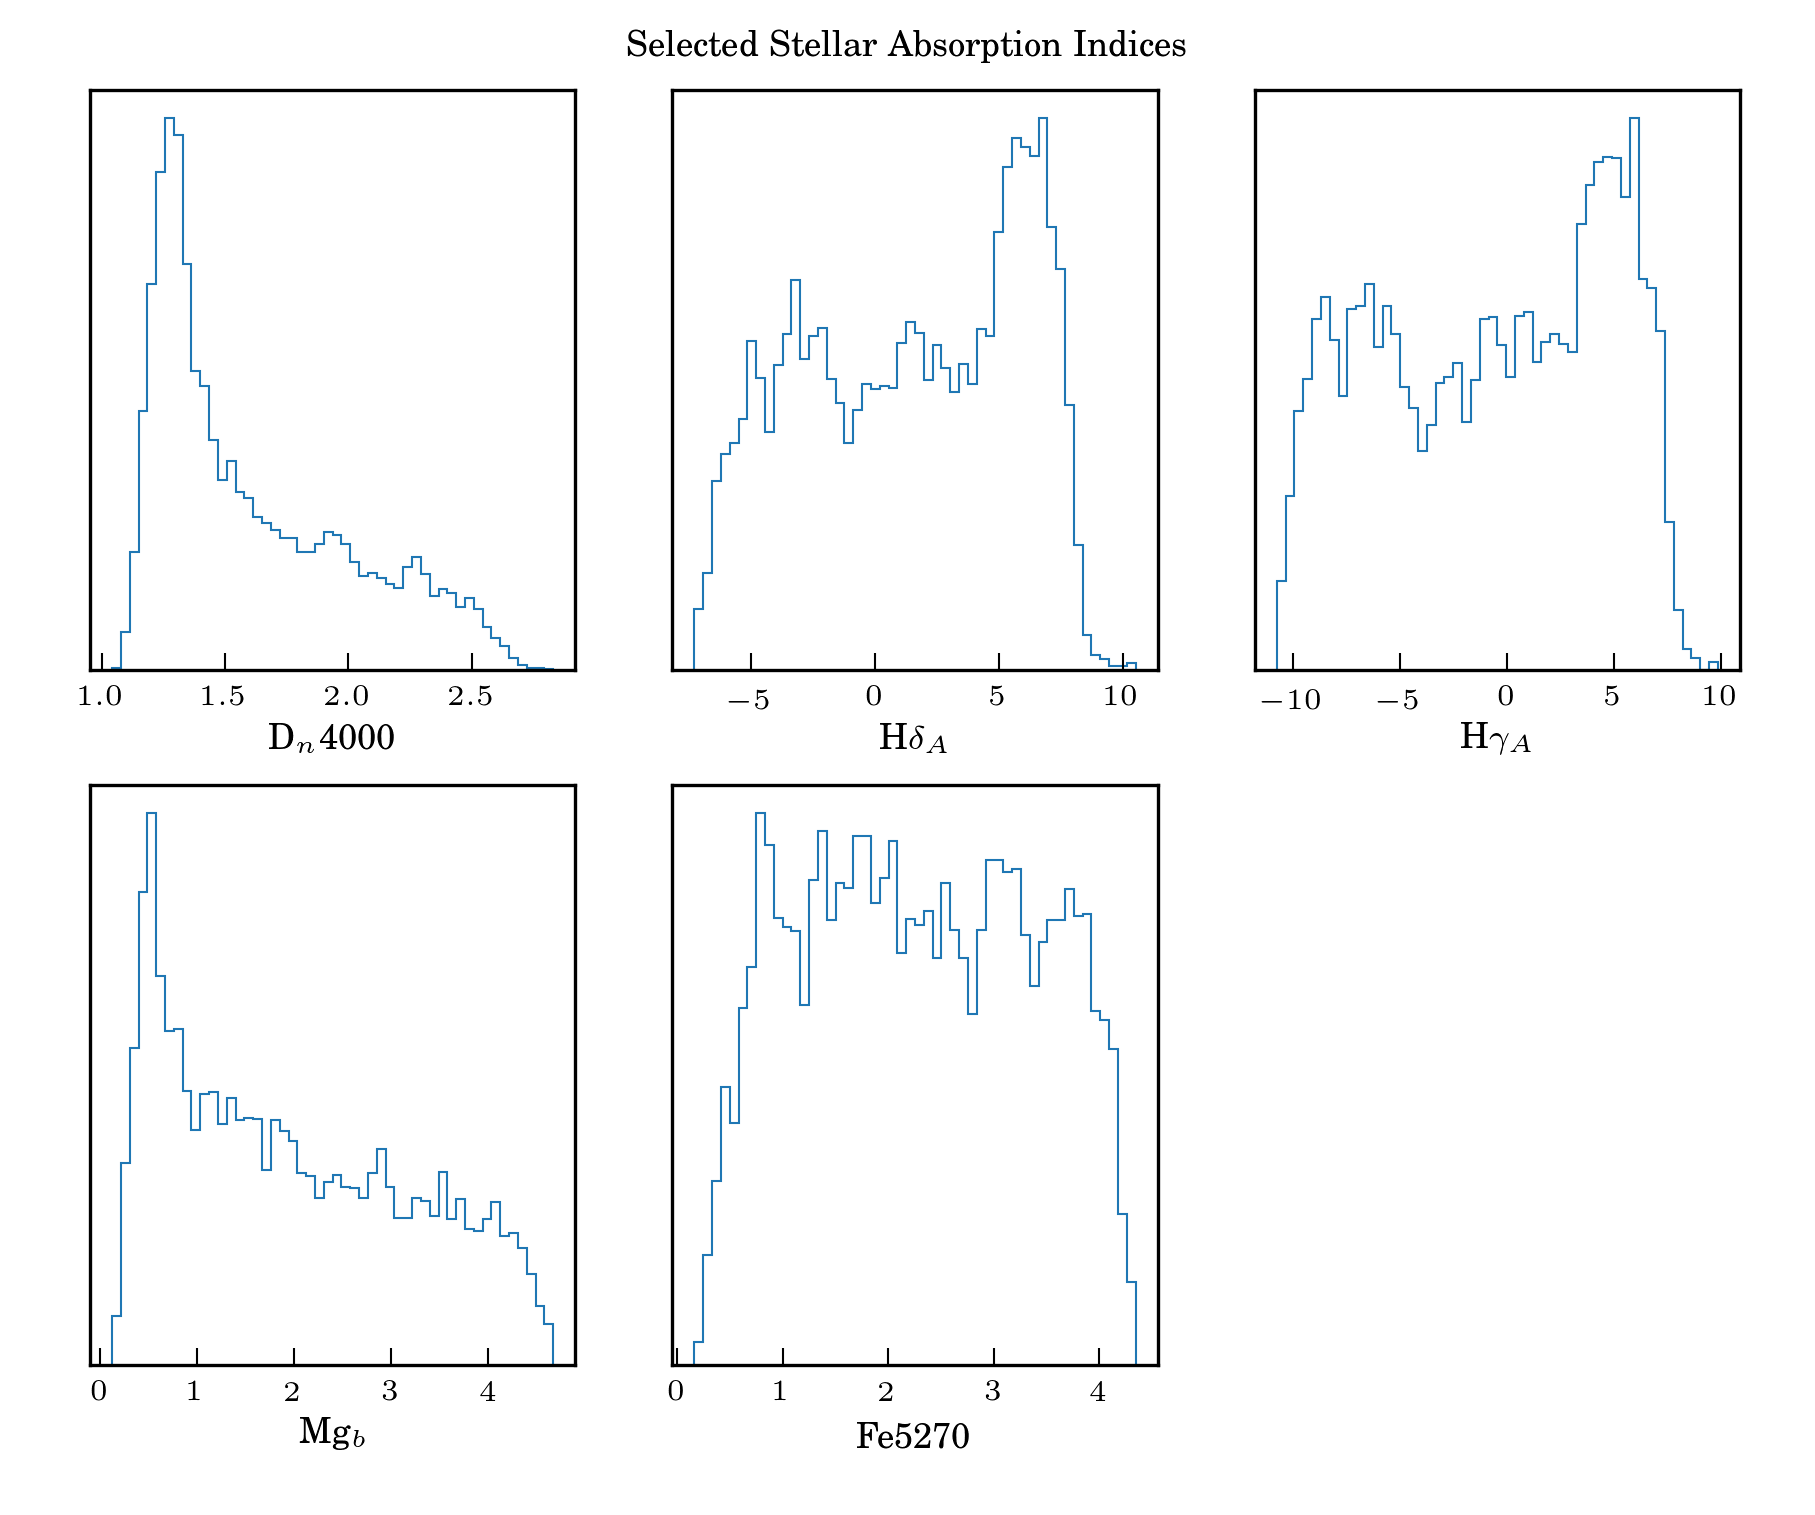
\includegraphics[width=\textwidth]{prior_specinds}
    \caption[Distributions of absorption indices in training data]{\fixspacing The distributions of five absorption indices in our synthetic training data: \Dn, \HdeltaA, \HgammaA, Mg$_b$, and Fe5270.}
    \label{fig:prior_specinds}
\end{figure*}

\begin{figure*}
    \centering
    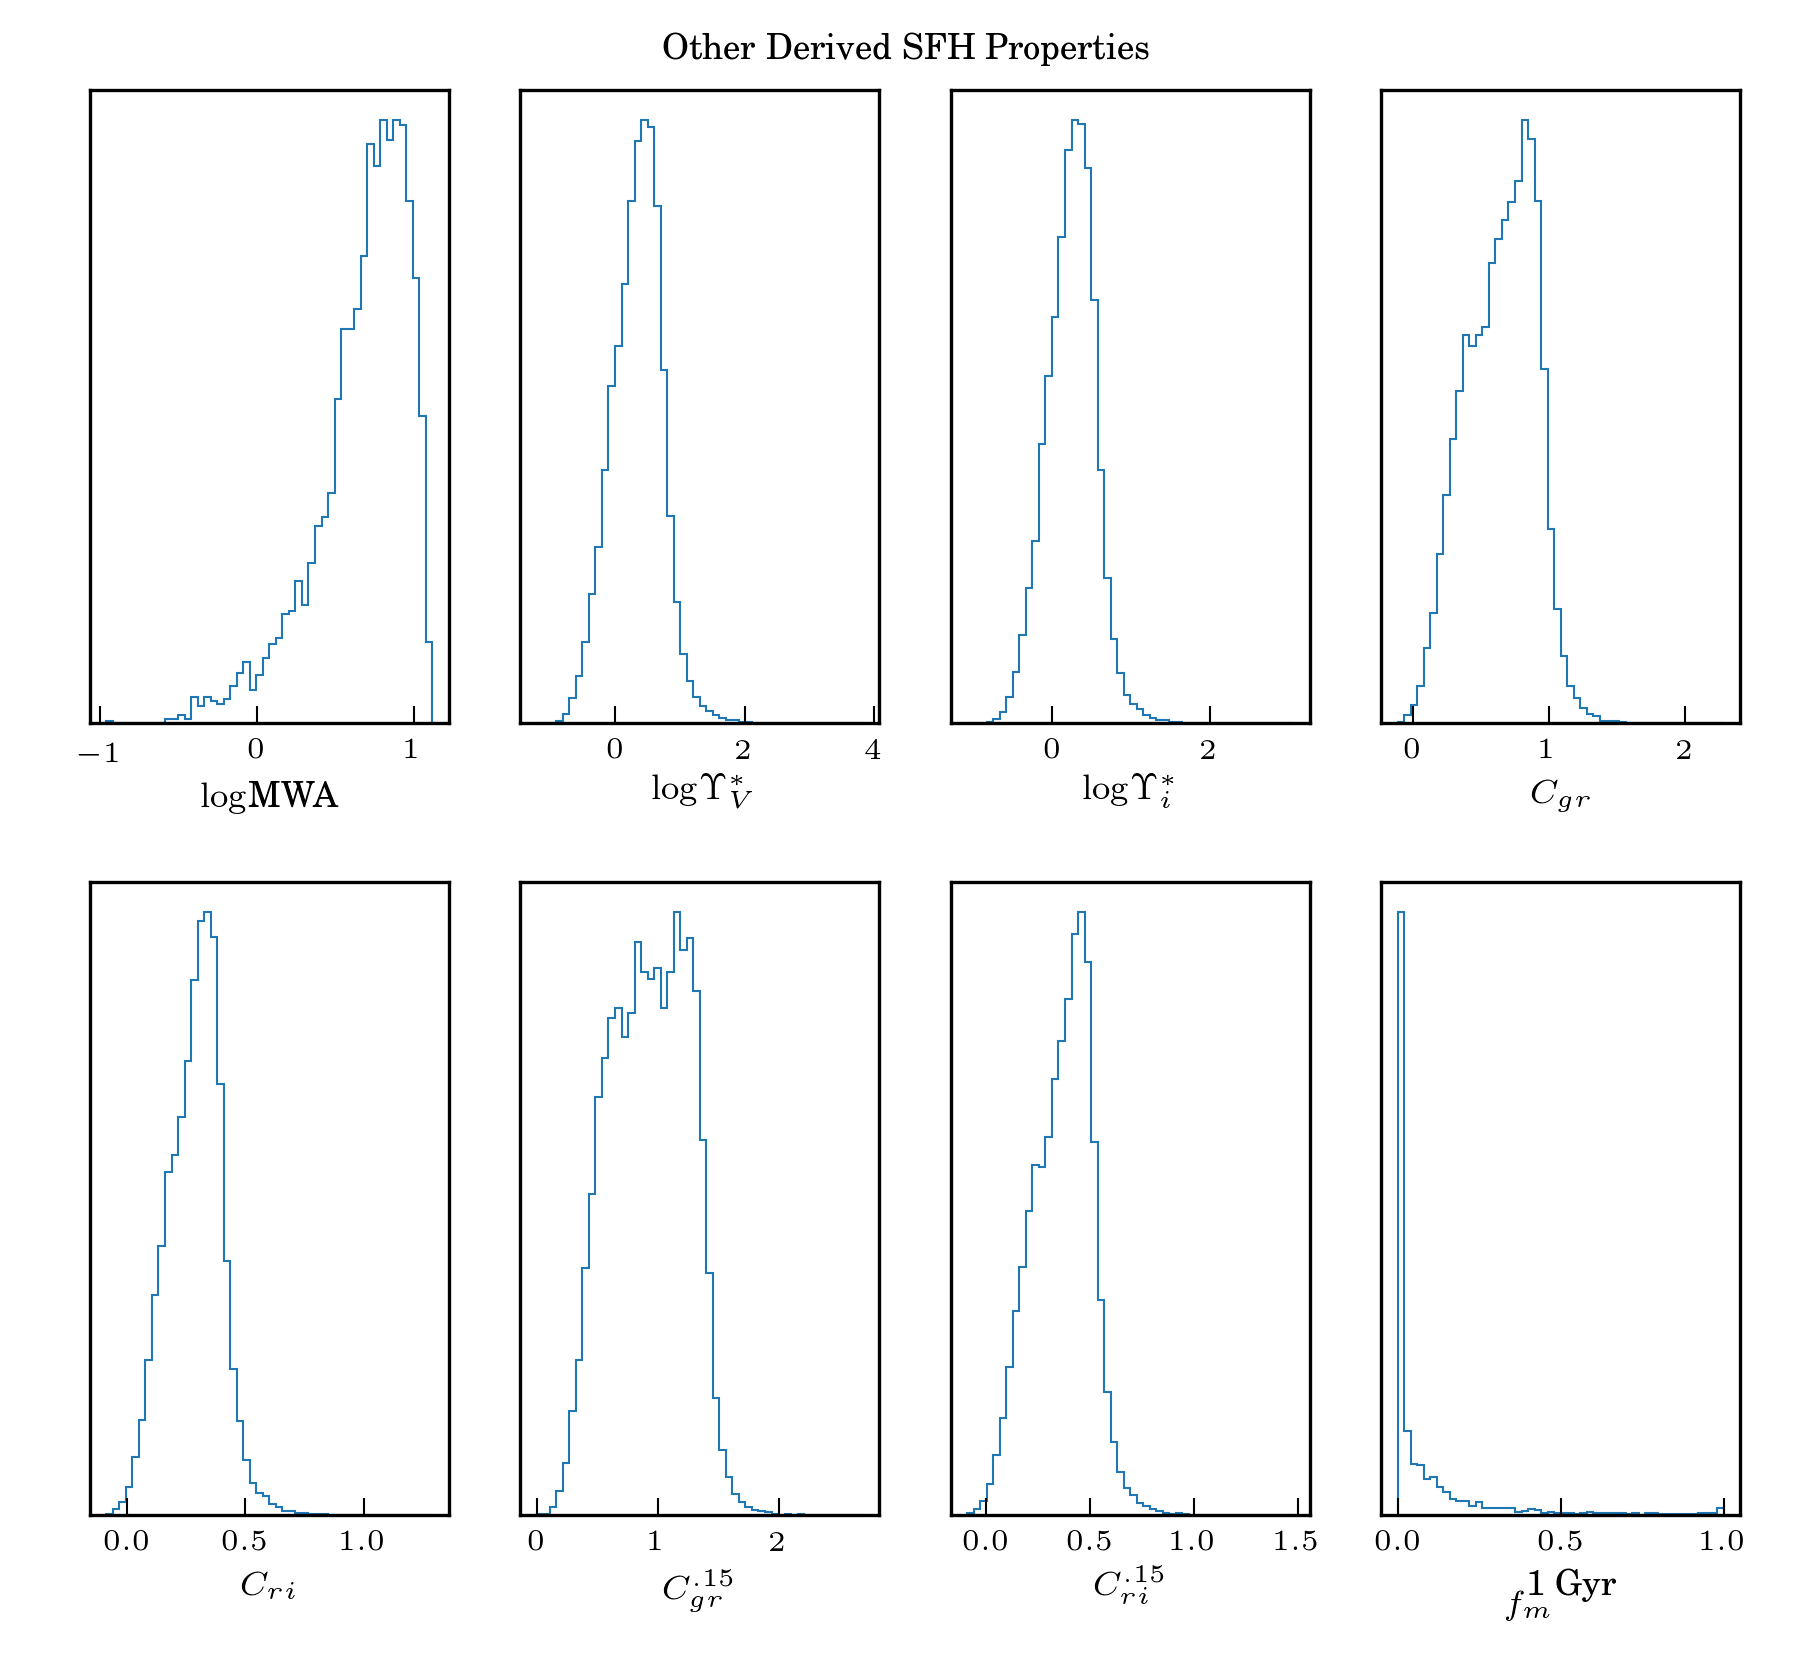
\includegraphics[width=\textwidth]{prior_otherderived}
    \caption[Distributions of derived SFH properties in training data]{\fixspacing The distributions of eight derived parameters which are secondarily obtained from the SPS, using the distributions of inputs shown in Figure \ref{fig:prior_inputparams}: mass-weighted stellar age, stellar mass-to-light ratios in $V$ \& $i$ bands, rest-frame $g-r$ and $r-i$ color, the same colors at redshift of 0.15, and fraction of stellar mass formed in the past 1 Gyr.}
    \label{fig:prior_otherderived}
\end{figure*}

\subsubsection{SFH families: the delayed-$\tau$ model}
\label{chap1:sec:SPS_params}

\citetalias{chen_pca} based the adopted family of SFHs on a tau (declining exponential) model: additionally, one or more stochastic bursts were permitted, and a fraction of SFHs cut off rapidly, in order to emulate post-starburst galaxies at high redshifts \citep{kriek_06, kriek_09}. However, merely allowing a \emph{cutoff} in the SFH does a poor job at reproducing the more vigorously-star-forming outer regions of disk galaxies, which do have older stars, but whose SFHs are shown in both observations and cosmological simulations to rise through the present day \citep{pacifici_12_SFHs,pacifici_13_SFHs}. \citet{simha_14_SFHs} found that a more flexible delayed-$\tau$ model (also referred to as ``lin-exp") plus stochastic bursts and an optional subsequent ramp up (rejuvenation) or down (cutoff) effectively decouples late from early star-formation, and provides a better fit to photometric data. As such, we adopt this slightly more complicated framework.

The most basic delayed-$\tau$ model is parametrized by a starting time (before which the SFH is identically zero) and an $e$-folding timescale (which sets the shape of the SFH). Each are drawn from a smooth distribution:

\begin{itemize}
\itemsep0em
    \item \emph{Formation time} ($t_{form}$), drawn from a normal distribution with mean of 5 Gyr and width of 4 Gyr, and which truncates below 0.2 Gyr and above 13.0 Gyr. This broad distribution is similar to the uniform distribution adopted in \citetalias{chen_pca}.
    \item \emph{e-folding timescale of the continuous component} ($\textrm{EFTU}$), which has a log-normal distribution centered at $\log \frac{\mu}{\rm Gyr} = 0.4$ and with $\log \frac{\sigma}{\rm Gyr} = 0.4$. The distribution truncates below 0.1 Gyr and above 15 Gyr. Since the peak of the $t e^{-t/\tau}$ has its peak at an interval $\tau$ after formation, this broad distribution of e-folding times allows SFHs that form quickly, as well as those that continue to rise until the present day.
\end{itemize}

The prevalence, duration, and strength of merger-induced bursts have been investigated in Tree-SPH and N-body sticky-particles simulations \citep{dimatteo_08}. Though such simulations lack the resolution to model gas cooling to molecular-cloud temperatures, they are useful simply as order-of-magnitude guidance. \citet{dimatteo_08} also found that most merger-driven bursts last several $10^8$ years, with the vast majority lasting less than 1 Gyr, which informs the upper-limit for burst duration shown below. \citet{gallazzi_bell_09} conclude that recent bursts are necessary to reproduce the full space of stellar absorption features, simultaneously warning that \textit{overestimating} the number of bursts could result in systematically-low mass-to-light ratios for galaxies dominated by a continuous SFH.

We express the strength of a burst in terms relative to the peak of the underlying lin-exp model: that factor is simply added to the latent SFR at all times in the range $[t_{burst}, t_{burst} + dt_{burst}]$. Finally, we note that we do not model stochastic, short-timescale (several to tens of Myr) variations in SFR, primarily due to computational concerns. Conceivably, for sufficiently young ($<$ 1 Gyr) stellar populations, anomalously-steady models (i.e., SFHs that are \emph{too smooth}) could induce a negative systematic in stellar mass-to-light ratio (effecting an additional, intrinsic scatter in the SFH parameter space). The bursts are generated according to the following randomized prescription:

\begin{itemize}
    \item \emph{Number of bursts} ($n_{bursts}$, an integer) giving the number of starbursts. The value is generated by a Poisson distribution with a mean and variance $\frac{0.5 \times (t_0 - \min(\{t_{t}), t_{form}\}))}{t_0}$. That is, if a SFH were to initiate immediately at $t=0~{\rm Gyr}$ and not be cut off, the average number of bursts would be 0.5. Functionally, most SFHs experience zero stochastic bursts, and the mean number of bursts per SFH is 0.256.
    \item \emph{Burst amplitudes} ($A$, a list with $n_{bursts}$ elements). Individual values in $A$ are distributed log-normally between 0.1 and 10, and indicate the addition of $A$ times the maximum value of the pure delayed-$\tau$ model during the times when the burst is active.
    \item \emph{Burst times} ($t_{burst}$, a list), whose length is the same as $A$, and whose elements are uniformly distributed between $t_{form}$ and $t_0$ (or $t_{t}$, if there is a cutoff).
    \item \emph{Burst duration} ($dt_{burst}$, a list) which specifies the duration for each burst, uniformly distributed between 0.05 and 1 Gyr. 
\end{itemize}

The delayed-$\tau$ model with bursts is further modulated by conservative allowances for a cutoff/rejuvenation at late times:

\begin{itemize}
    \item \emph{Transition probability} ($p_t$), a 25\% chance of either a rejuvenation or a cutoff in the SFH at time $t_t$, under the assumption that most SFHs are smoothly-varying.
    \item \emph{Transition time} ($t_{t}$), after which star formation may occasionally (as dictated by $p_t$) cut off or revive. This may occur with equal probability after $t_{form} + EFTU / 4$ until the present day (at the smallest allowable value, such a SFH functions like a brief starburst which could last as little as 25 Myr). If $p_t$ dictates there is no burst, $t_t$ is set to the age of the universe, and thus never impacts the SPS.
    \item \emph{Transition strength} $\theta$, specifying an ``angle" in time-SFR space, such that $\theta = 0$ corresponds to a SFR held constant after $t_t$ and $\theta = \frac{\pi}{2}$ corresponds to an immediate cutoff in the SFH. $\theta$ is distributed according to a triangular distribution rising from zero in the domain $\frac{\pi}{2} < \theta \le 0$, and falling back to zero in the domain $0 < \theta \le \frac{\pi}{6}$. If $p_t$ dictates there is no burst, $\theta$ is set to zero, but does not impact the SPS because $t_t$ is set to the age of the universe.
    \item \emph{Cutoff slope} is an $\arctan$-re-parametrization of $\theta$, scaled in units of the maximum of a pure delayed-$\tau$ model $\Phi_{max}$ per Gyr. Therefore, $\gamma = 0$ corresponds to a perfectly constant SFR after $t_t$, and $\gamma = -1.0$ to a reduction in the SFR by $\Phi$ in 1 Gyr.
\end{itemize}

These specific parameter distributions were chosen to produce the best match to the joint distribution of moderate- and high-signal-to-noise MaNGA spectra in \Dn-\HdeltaA space (see Section \ref{chap1:subsubsec:Dn4000-HdA_comp}). Compared with \citetalias{chen_pca}, $t_{form}$ is peaked more strongly at intermediate times, and ${\rm EFTU}$ is permitted to be less than 1 Gyr (and indeed, $\sim 40\%$ are). Additionally, starbursts occur on average less frequently in this work, but with stronger amplitude, since \citetalias{chen_pca} considered spatially-unresolved spectra (whose bursts have been ``spatially-averaged" to a greater probability, but lower mean strength). A sample of ten SFHs, drawn randomly from this prescription, is shown in Figure \ref{fig:sample_sfhs}.

Previous analyses of SDSS central spectroscopy have derived distributions of mass-weighted mean stellar age (MWA) for galaxies in the nearby universe: for example, \citet{gallazzi_charlot_05}, following \citet{kauffmann_heckman_white_03}, reports a distribution of mass-weighted mean stellar age (MWA) derived from fits to high signal-to-noise spectra. The \citet{gallazzi_charlot_05} MWA distribution strongly resembles the distribution from this work's model library (Figure \ref{fig:mwa_dist}). This work's model library has a more probable low-MWA tail, and a significantly younger mode. As the galaxy disks sampled by MaNGA have a diversity of ages (both young and old) compared to the central regions sampled in \textsc{SDSS-i} spectroscopy, this is a positive characteristic. The model MWA distribution from this work also bears similarity to the MWA distribution derived from integrating the \citet{madau_dickinson_2014_csfrd} cosmic star formation rate density: \citet{madau_dickinson_2014_csfrd} report a young-age tail, which this work's prior easily encompasses, but has a mode at nearly 10Gyr (about twice as old as the mode of this work's model libraries). No value judgment is made here regarding a particular MWA distribution; that said, noting MWA distributions' changes in shape resulting from manipulating the CSP inputs has proven informative in constructing a flexible training library.

\begin{figure}
    \centering
    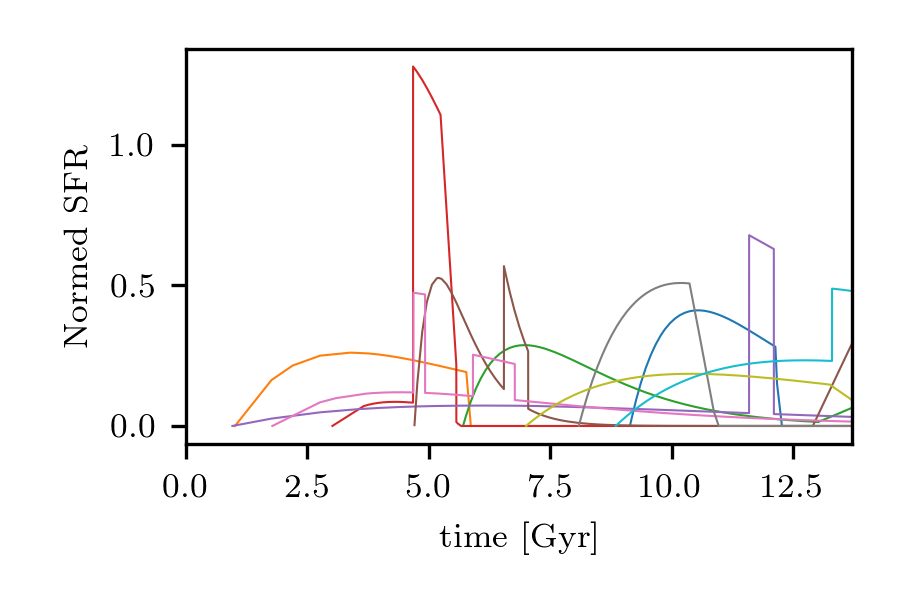
\includegraphics[width=\columnwidth]{randomSFHs}
    \caption[Ten sample SFHs]{\fixspacing Ten sample SFHs generated using the random prescription given in Section \ref{chap1:sec:SFHs}.}
    \label{fig:sample_sfhs}
\end{figure}

\definecolor{mplc0}{HTML}{1f77b4}
\definecolor{mplc1}{HTML}{ff7f0e}
\definecolor{mplc2}{HTML}{2ca02c}
\definecolor{mplc3}{HTML}{962728}
\definecolor{mplc4}{HTML}{9467bd}
\definecolor{mplc5}{HTML}{8c564b}
\definecolor{mplc6}{HTML}{e377c2}
\definecolor{mplc7}{HTML}{7f7f7f}
\definecolor{mplc8}{HTML}{bcbd22}
\definecolor{mplc9}{HTML}{17becf}

\begin{table*}
    \centering
    \begin{tabular}{||c|c|c|c|c||} \hline \hline
        Line color & $t_f$ & EFTU & $t_t$ & $\theta$ \\ \hline
        \textcolor{mplc0}{\texttt{C0}} (Tableau Blue) & 9.14 & 1.40 & 12.13 & -1.36 \\ \hline
        \textcolor{mplc1}{\texttt{C1}} (Tableau Orange) & 1.01 & 2.38 & 5.78 & -1.43 \\ \hline
        \textcolor{mplc2}{\texttt{C2}} (Tableau Green) & 5.71 & 1.27 & 13.01 & 0.13 \\ \hline
        \textcolor{mplc3}{\texttt{C3}} (Tableau Red) & 3.02 & 1.29 & 5.25 & -0.70 \\ \hline
        \textcolor{mplc4}{\texttt{C4}} (Tableau Purple) & 0.96 & 5.18 & 7.10 & -0.04 \\ \hline
        \textcolor{mplc5}{\texttt{C5}} (Tableau Brown) & 4.71 & 0.50 & 12.90 & 0.13 \\ \hline
        \textcolor{mplc6}{\texttt{C6}} (Tableau Pink) & 1.78 & 2.61 & - & - \\ \hline
        \textcolor{mplc7}{\texttt{C7}} (Tableau Gray) & 8.09 & 2.10 & 10.37 & -0.92 \\ \hline
        \textcolor{mplc8}{\texttt{C8}} (Tableau Olive) & 7.00 & 3.39 & 13.25 & -0.59 \\ \hline
        \textcolor{mplc9}{\texttt{C9}} (Tableau Cyan) & 8.85 & 3.88 & - & - \\ \hline
    \end{tabular}
    \caption[Selected parameters for ten sample SFHs]{\fixspacing Selected CSP parameters for the SFHs shown in Figure \ref{fig:sample_sfhs}. For each CSP, we list the line color, the formation time $t_f$, the e-folding time of the continuous component (EFTU), the transition time $t_t$, and the transition strength $\theta$. Models with no transition behavior have the $t_t$ and $\theta$ columns left blank.}
    \label{tab:sfh_params}
\end{table*}

\begin{figure}
    \centering
    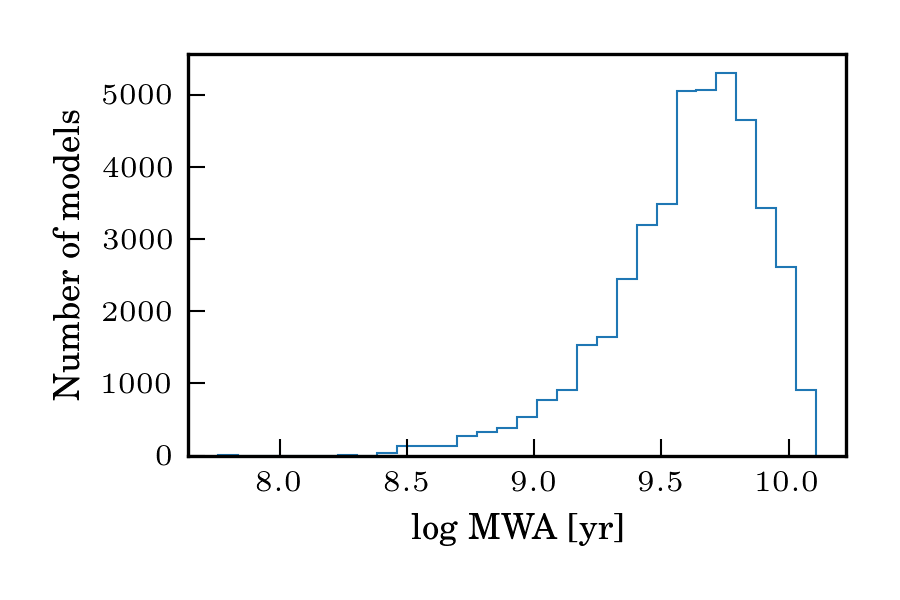
\includegraphics[width=\columnwidth]{MWA_dist}
    \caption[Distribution of the log mass-weighted mean stellar age for training data]{\fixspacing The distribution of the log of mass-weighted mean stellar age for all of the template SFHs. As in \citet{gallazzi_brinchmann_08}, the distribution has a broad peak around $\log {\rm MWA} \sim 9.8$. Unlike \citet{gallazzi_brinchmann_08}, though, the distribution extends with significant power below $\log {\rm MWA} \sim 9.0$, meaning that more recent star-formation is permitted.}
    \label{fig:mwa_dist}
\end{figure}

\subsubsection{Stellar composition \& velocities, attenuation, and uncertain stellar evolution}

Since the star-forming ISM is known to enrich with heavy elements as successive generations of stars form, it is most correct to consider both a metallicity history and a star formation history. Though gaseous emission captures the current enrichment state, it is subject to significant differences in interpretation, including concepts as fundamental as the zeropoint \citep{stasinska_07_review}. Certain stellar absorption indices, particularly those targeting magnesium \citep{barbuy_92}, reflect the average enrichment state of the stars. However, the Mg-based indices in particular are not reliable at low metallicity \citep{maraston_03b}. In addition, there is some evidence that when trying to fit a population with known-evolving metallicity using a single, non-evolving stellar metallicity, absorption index-based estimates of stellar mass-to-light ratio suffer from smaller biases than do color-based estimates. This is because stellar mass-to-light ratio varies in the \Dn--\HdeltaA plane in a very similar way, when fixed- and evolving-metallicity populations are compared \citep[see][Section 5]{gallazzi_bell_09}. Finally, in order to properly consider a SFH with an evolving metallicity, additional parameters must be introduced to capture inflows, outflows, and feedback \citep{matteucci_16_chemev}. Section \ref{chap1:subsubsec:Dn4000-HdA_comp} briefly outlines a comparison made between spectral indices such as \Dn and \HdeltaA measured in the models and in the observations, and supports the assertion that non-evolving metallicities suffice for our purposes.

With these considerations in mind, we do not implement any chemical evolution prescription, instead adopting SFHs with non-evolving stellar metallicities. Each SFH model is assigned a single metallicity $[Z]$, constant through time, which has an 80\% chance to be drawn from a metallicity distribution that is linearly-uniform, and a 20\% chance to be drawn from a metallicity distribution that is logarithmically-uniform. This allows a small, but well-populated low-metallicity tail. Figure \ref{fig:metallicity_prior} compares the gas-phase oxygen abundance from the SDSS MPA-JHU catalog \citep{tremonti_mz} to the adopted metallicity prior, after a zeropoint normalization \citep{asplund_09}. These distributions should be (and are) roughly similar, since the chemical composition of the gas reflects how baryons are cycled through stars and enriched successively by several generations of star-formation.

\begin{figure}
    \centering
    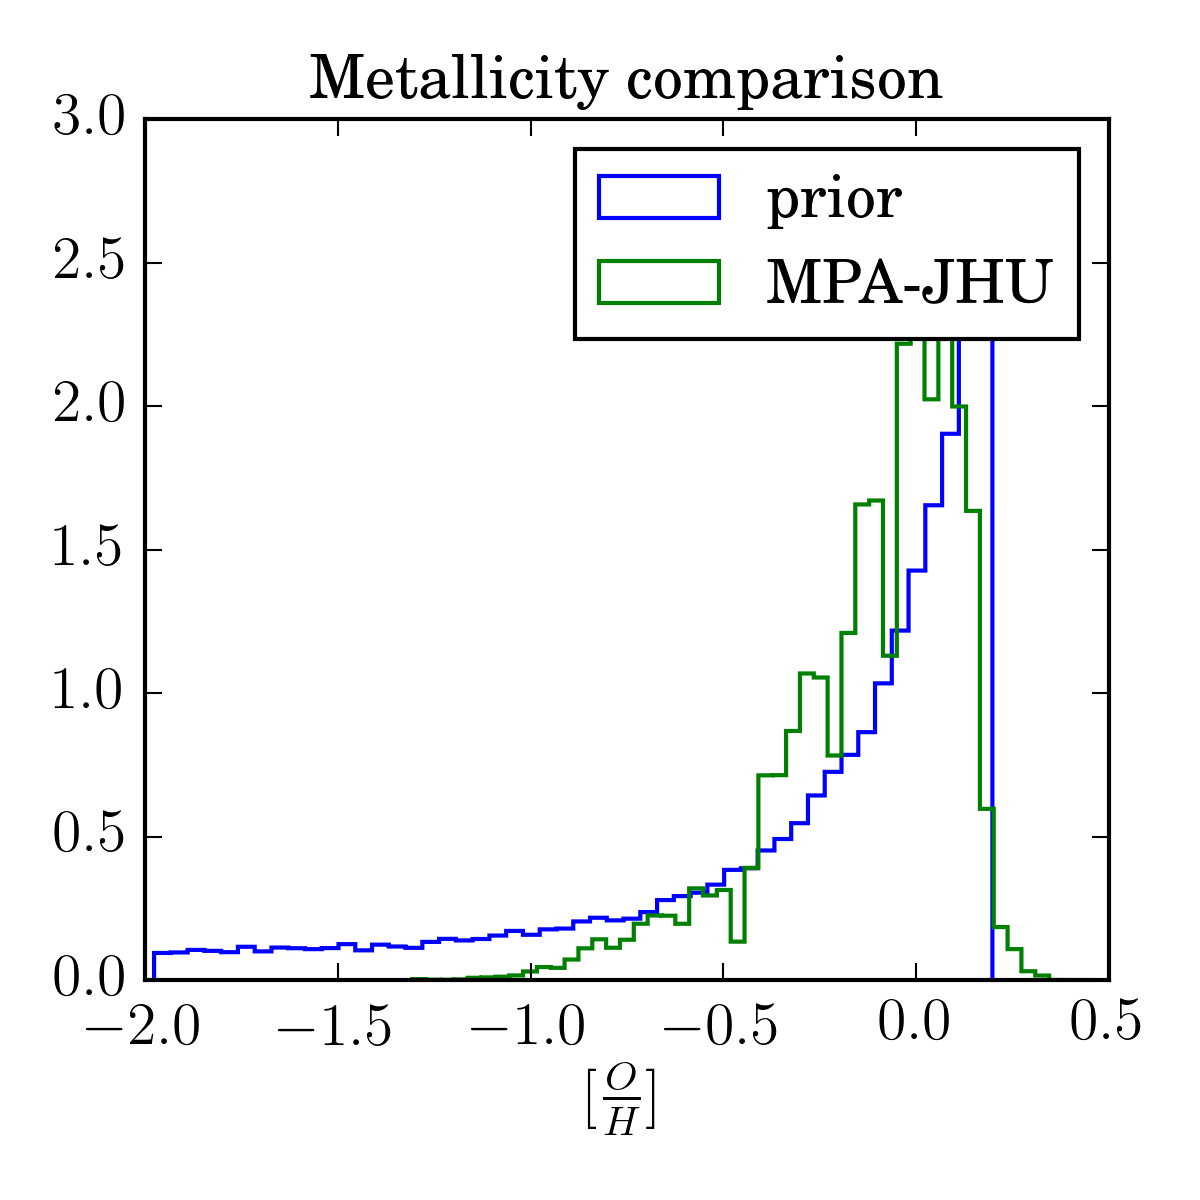
\includegraphics[width=\columnwidth]{metallicity-prior}
    \caption[Comparison of SDSS nebular metallicity distribution with training data stellar metallicity distribution]{\fixspacing Comparison of the solar-normalized oxygen abundance ($[\frac{O}{H}]$) inferred from SDSS nebular emission (\textit{green}) with the adopted metallicity prior. An offset of approximately -.29 dex is applied to re-scale the  SFH library's metallicity range ($[Z]$, based on mass) to the number-abundance of oxygen from the SDSS data, since the two adopt different values of solar metallicity and oxygen abundance.}
    \label{fig:metallicity_prior}
\end{figure}

Two uncertain phases of stellar evolution, blue horizontal branch (BHB) and blue straggler stars (BSS), are also modulated in prevalence: while they can affect stellar mass-to-light ratio estimates by $\sim$ 0.1 dex for the intermediate-age populations found in galaxy disks \citep{fsps_1}, there are precious few precise enough measurements of either of their abundances to inform this work's CSP library. Adopting smooth and permissive priors for these less-well-constrained parameters avoids unjustified restrictions on the resulting spectral fits. In reality, we are in most cases unable to further constrain these parameters based on our fits to spectra (see Section \ref{chap1:sec:method} and Appendix \ref{chap1:apdx:fakedata}), but we also lack the observational constraints from stellar-evolution to choose one value in particular.

While BHB stars are likely more common at low metallicity, it is inadvisable to neglect them for other cases \citet{fsps_1}. As such, we draw their fraction by number ($f_{BHB}$) from a beta-distribution with shape parameters $\alpha=2$ and $\beta=7$: this distribution is restricted to lie between zero and one, and represents a plausible range of BHB incidence rates. Specific BSS frequency ($S_{BSS}$, defined with respect to \emph{all} horizontal branch stars) is known to vary somewhat with environment, but is not constrained well in an absolute sense by observations \citep{santucci_2015_BSS}. The binary mass-transfer pathway for BSS formation \citep{gosnell_14_bluestraggler} implies that any factors (e.g., environment or metallicity) affecting star formation could also manifest in the BSS population. Furthermore, \citet{piotto_04_bluestraggler} noted that BSS frequency is lower in clusters than in the field, in a way not explained by the expected increased collision rates in clusters. As such, we adopt a broad distribution, 10 times the value of a draw from a beta distribution with shape parameters $\alpha=1$ and $\beta=4$---which allows the full range of 0.0--0.5 adopted by \citet{fsps_1}, is more permissive at the high end than the estimates of \citet{dorman_95}, and peaks at approximately 0.2.

Attenuation of the starlight is accomplished using a two-component dust model \citep{charlot_fall_00}. In this model, all stars are attenuated by diffuse dust with a V-band optical depth $\tau_V \mu$ and power-law slope of -0.7 \citep[as in][]{chevallard_charlot_16_beagle, da-cunha_charlot_elbaz_08}; while stars younger than 10 Myr are further attenuated by the dense ISM with optical depth $\tau_V (1 - \mu)$ and power-law slope of of -1.3. Therefore, a young stellar population will in total experience an optical depth of $\tau_V$, discounting effects resulting from different dust law slopes. In our schema, $\tau_V \mu$ and $\mu$ are randomized directly (rather than $\tau_V$ and $\mu$ individually), because all stellar populations experience $\tau_V \mu$, meaning that it is a more effective parameter most of the time:

\begin{itemize}
    \itemsep0em
    \item The \emph{product} $\tau_V \mu$ is drawn from a normal distribution with mean 0.4 and standard deviation 0.2, truncated at 0 and 1.2.
    \item \emph{Fractional optical depth of the diffuse ISM} ($\mu$), drawn from a normal distribution with mean of 0.3 and standard deviation of 0.2, truncated at 0.1 and 0.9.
    \item \emph{Optical depth of young birth clouds} ($\tau_V$), the quotient $\frac{\tau_V \mu}{\mu}$.
\end{itemize}

These distributions were chosen such that their means correspond roughly to the ``standard" values given in \citet{charlot_fall_00}, with significant latitude to allow for both unobscured and highly-obscured stellar populations. The overall distribution has a similar mode to, but is broader (i.e., more permissive at the high end) than the attenuation distribution for star-forming galaxies found in \citet{brinchmann_04_mpajhu} by fitting emission lines with photoionization models.

Stellar velocity dispersion ($\sigma$) is also varied, and is drawn from a truncated exponential distribution with lower-limit of 10 km s$^{-1}$, upper-limit of 350 km s$^{-1}$, and e-folding scale of 350 km s$^{-1}$. This is intended to populate both the low-$\sigma$ stellar disk and the high-$\sigma$ bulge. This does not include the wavelength- and redshift-varying contribution of the instrumental line-spread function (LSF), which is accounted for separately (see Appendix \ref{chap1:apdx:lsf}).

Each SFH is initialized with several different sets of dust properties ($\tau_V$ and $\mu$) and velocity dispersion ($\sigma$), for computational reasons. In addition to easing the processing load, this ensures a complete population of the parameter space at significantly lower computational cost (in total, \nSFHs CSPs were generated, each of which has \nsubsample combinations of attenuation and velocity dispersion.) Subsampling in velocity dispersion and attenuation becomes important to ensure that enough models fit the data well enough to perform good parameter inference: in Appendix \ref{chap1:apdx:fakedata}, we use additional synthetic data (i.e., ``held-out data" generated identically to the training spectra but not included in PCA training) to test the reliability of our stellar mass-to-light estimates against mock galaxies with known physical properties; and in Section \ref{chap1:subsubsec:Dn4000-HdA_comp}, we compare the distribution of all of the training data in \Dn and \HdeltaA to empirical measurements of the same indices from many thousands of spectra reported in the MaNGA DAP, demonstrating that other than one small, well-known systematic affecting \HdeltaA at moderate \Dn, the training models are distributed very similarly to empirical measurements of \Dn and \HdeltaA in observed spectra.

For each model, the SFH is stored (as it is used explicitly by \texttt{FSPS}), along with the strengths of several spectral absorption indices\footnote{All stellar absorption indices are computed on spectra with velocity dispersion of $\sigma$ = 65 km s$^{\rm -1}$, approximately equal to the difference in resolution between full-resolution model spectra and MaNGA data. This is preferable to employing correction factors which are not guaranteed to work for stellar populations younger than 3 Gyr \citep{kuntschner_04_lick_losvd_corr}.}, the mass-weighted age, and $V$- \& $i$-band mass-to-light ratios ($\Upsilon^*_V$ \& $\Upsilon^*_i$)\footnote{\emph{Effective} mass-to-light ratios are used, since they include only light that reaches the observer. In other words, these effective mass-to-light ratios are affected by dust. All subsequent references to mass-to-light ratio use this same abbreviation. For the purposes of estimating stellar mass, though, this convention suffices, because the bandpass flux which is multiplied by the mass-to-light ratio and the distance modulus \emph{also} is attenuated by dust, so the two dust contributions cancel.}.

\subsection{\Dn-\HdeltaA comparison of training library to MaNGA spaxels}
\label{chap1:subsubsec:Dn4000-HdA_comp}

We evaluated the correspondence between the suite of synthetic models and the real MaNGA data by comparing the distribution of the \Dn and \HdeltaA absorption indices measured by the MaNGA DAP to those from the full suite of SFH models (the ``training data") used in this work (Figure \ref{fig:CSP+lowZ_SSP_mf03}). We observe an offset in \HdeltaA between synthetic models and observations at fixed \Dn greater than 1.5, consistent with previous work \citep[see][Figure 2]{kauffmann_heckman_white_03}. This effect has been attributed to stellar models, and the offset observed (which grows with \Dn, but remains less than 0.8 $\mbox{\AA}$) is well within the locus of previous measurements. Some degree of this offset may be attributable to $\alpha$-enhancement, which cannot be manipulated in the set of stellar atmospheres adopted for this work. It is likely that such a mismatch exists at all values of \Dn, but becomes apparent only at \Dn $>$ 1.5---that is, at ages of several Gyr (where CSPs with e-folding timescales shorter than 1Gyr begin to have similar spectra to SSPs).

Furthermore, though \citet{maraston_stromback_09} finds that superimposing approximately 3\% (by mass) of low-metallicity stars onto synthetic continuous stellar populations can resolve a color mismatch between synthetic CSP models and luminous red galaxies (LRGs), we find no evidence for a similar improvement in the case of \Dn and \HdeltaA (in Figure \ref{fig:CSP+lowZ_SSP_mf03}, we show the case where the mass fraction is 3\%). We observe, though we do not show, that as the mass fraction of the SSP increases, the value of \HdeltaA actually \emph{decreases} at fixed \Dn. That said, \citet{maraston_stromback_09} note that a potential astrophysical reason for the bluer-than-anticipated colors in metal-poor galaxies is an especially strong blue horizontal branch, which is manipulated separately in our population synthesis. Finally, since the fraction of MaNGA spaxels that lie in the centers of massive LRGs is low, any effect of mixed-metallicity populations may be subdominant to others which pertain to more star-forming systems.

\begin{figure*}
    \centering
    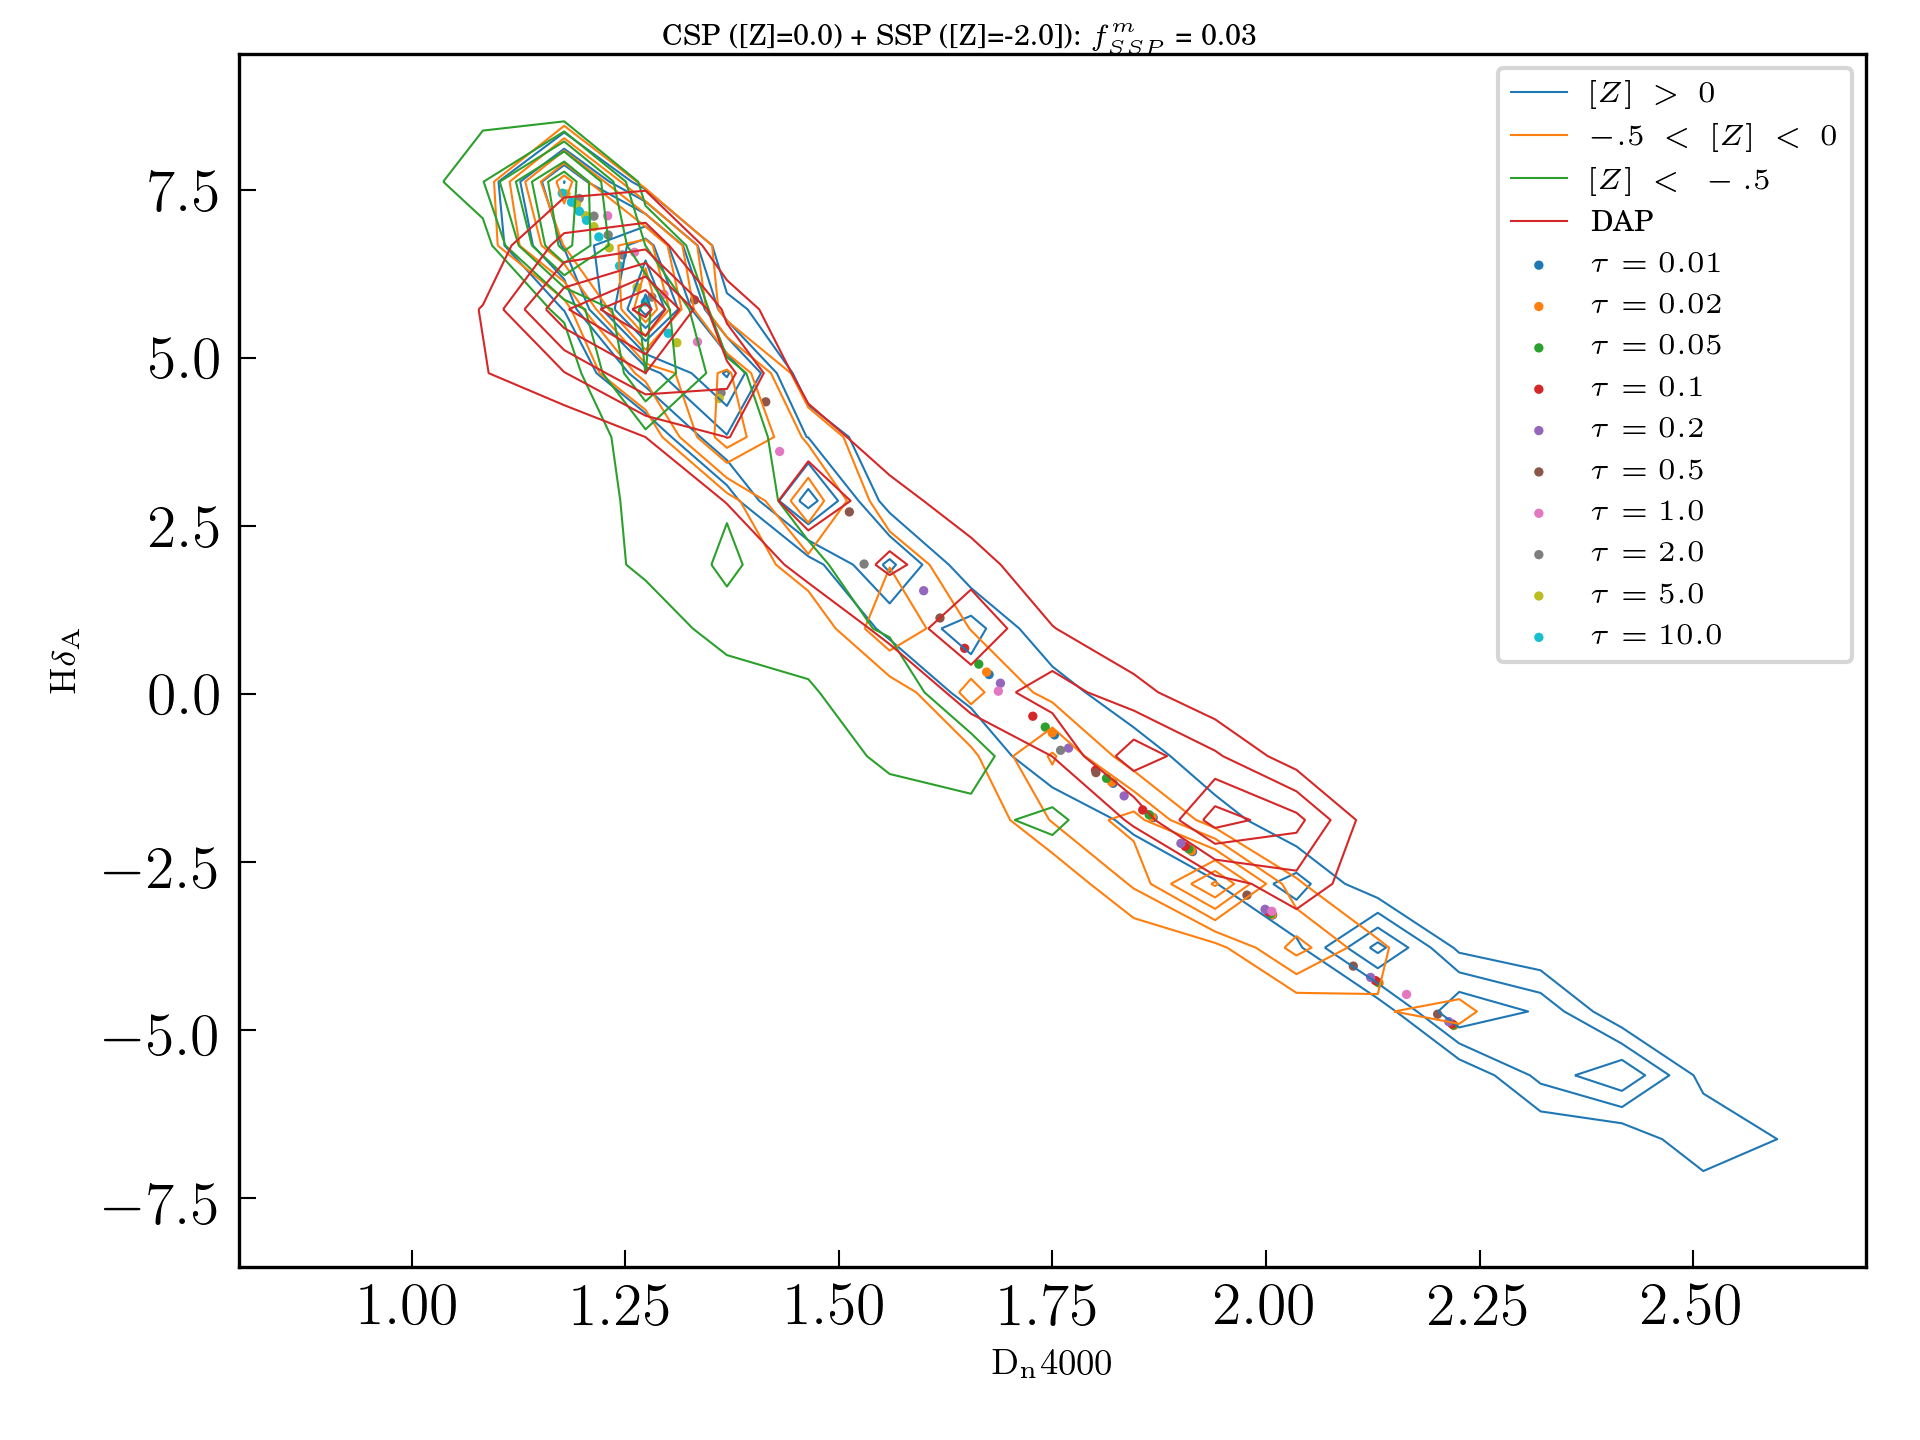
\includegraphics[width=\textwidth]{CSPs+lowZ_SSP_mf03}
    \caption[\Dn-\HdeltaA comparison between training data, MaNGA DAP values, and a set of expanded models]{\fixspacing The distribution of the training models in \Dn-\HdeltaA space (separated by stellar metallicity: super-solar metallicity in blue contours, slightly sub-solar in orange contours, and very sub-solar in green contours); plus data points for individual models with composite metallicities. Each point signifies a delayed-tau model with time constant denoted by the color of point (but forming at a variety of times post-Big-Bang). The continuous portion of the model is fixed at solar metallicity. Added to this CSP is a SSP which forms instantaneously at the same time as the CSP begins to form stars, with a contribution to the current stellar mass of 3\%. The SSP has an extremely low metallicity (${\rm [Z]}$ = -2).}
    \label{fig:CSP+lowZ_SSP_mf03}
\end{figure*}

An attempt to replace \HdeltaA with the sum of \HdeltaA and \HgammaA in lieu of just \HdeltaA, since a deficiency in \HgammaA has been noted to function opposite to a deficiency in \HdeltaA. In reality, the match is not greatly improved.

\subsection{Why not use CMLRs?}
\label{chap1:subsec:cmlrs}

\citet{bell_03} produced conversions between various optical colors and mass-to-light ratio, and we will re-evaluate this approach here. Table \ref{tab:bell_vs_here} compares the inputs to the stellar population synthesis modelling used to derive the \citet{bell_03} CMLRs, to the inputs used in this work. Salient differences include this work's modest allowances for starbursts, inclusion of attenuation---previously argued to be unimportant, due to the slope of the reddening vector being very similar to the CMLR \citep{bell_dejong_01, bell_03}---, and use of the \citet{kroupa_imf_01} IMF.

\begin{table*}
    \centering
    \begin{tabular}{||c||p{1.5in}|p{1.5in}|p{1.5in}||} \hline
        Input & \citet{bell_03} & \citet{taylor_gama_cmlrs} & This Work \\ \hline 
        Stellar models & P\'{E}GASE \citep{fioc_97_pegase} & \citet{BC03} & \citet{fsps_c3k} \\ \hline 
        Stellar IMF & ``Diet" \citet{salpeter_imf_55}---also see \citet{bell_dejong_01} & \citet{chabrier03} & \citet{kroupa_imf_01} \\ \hline 
        SFHs & delayed-$\tau$ & $\tau$-model, grid-sampled & Composite: delayed-$\tau$, burst(s), cutoff, rejuvenation \\ \hline 
        Attenuation & None & Uniform screen & Two-component \citep{charlot_fall_00} \\ \hline 
    \end{tabular}
    \caption[Population synthesis inputs of this work, compared to previous]{\fixspacing SPS inputs, compared between \citet{bell_03}, \citet{taylor_gama_cmlrs}, and this work.}
    \label{tab:bell_vs_here}
\end{table*}

Using the training data described above, we use a least-squares fit to find the optimal CMLR for $i$-band stellar mass-to-light ratio and both $g-r$ and $g-i$ colors---the latter being provided as a point of comparison to the GAMA survey \citep{taylor_gama_cmlrs}---and then examine the mean absolute deviation between the predicted and actual values of $\log \Upsilon^*_i$ (Figures \ref{fig:CMLR_Cgr-MLi-dev} and \ref{fig:CMLR_Cgi-MLi-dev}). As Figures \ref{fig:CMLR_Cgr-MLi-dev} and \ref{fig:CMLR_Cgi-MLi-dev} illustrate, our models follow a well-defined CMLR, but with a scatter of at 0.05--0.1 dex about the best-fit: scatter is lowest at modest values of stellar attenuation and sub-solar metallicities (the $g-i$ CMLR is slightly better in this respect). Furthermore, the CMLRs rely upon nearly perfect photometry, which in reality rarely improves to sub-0.02 levels at kiloparsec sampling scales for large surveys. That is, depending on the precise choice of CMLR, observational effects can very easily add further uncertainties of $\sim$0.05 dex. The differences between the \citet{bell_03}, \citet{taylor_gama_cmlrs}, and this work's CMLRs are not insubstantial: \citet{bell_03} CMLRs have uniformly smaller slope, meaning that they will produce mass estimates that are higher (lower) for blue (red) colors. In contrast, stellar mass-to-light ratios from the \citet{taylor_gama_cmlrs} CMLR will be uniformly lower than this work's, by 0.15--0.4 dex. This highlights the impact of the specific SFH family chosen, the stellar models, and even the choice of attenuation (see below).

\begin{figure*}
    \centering
    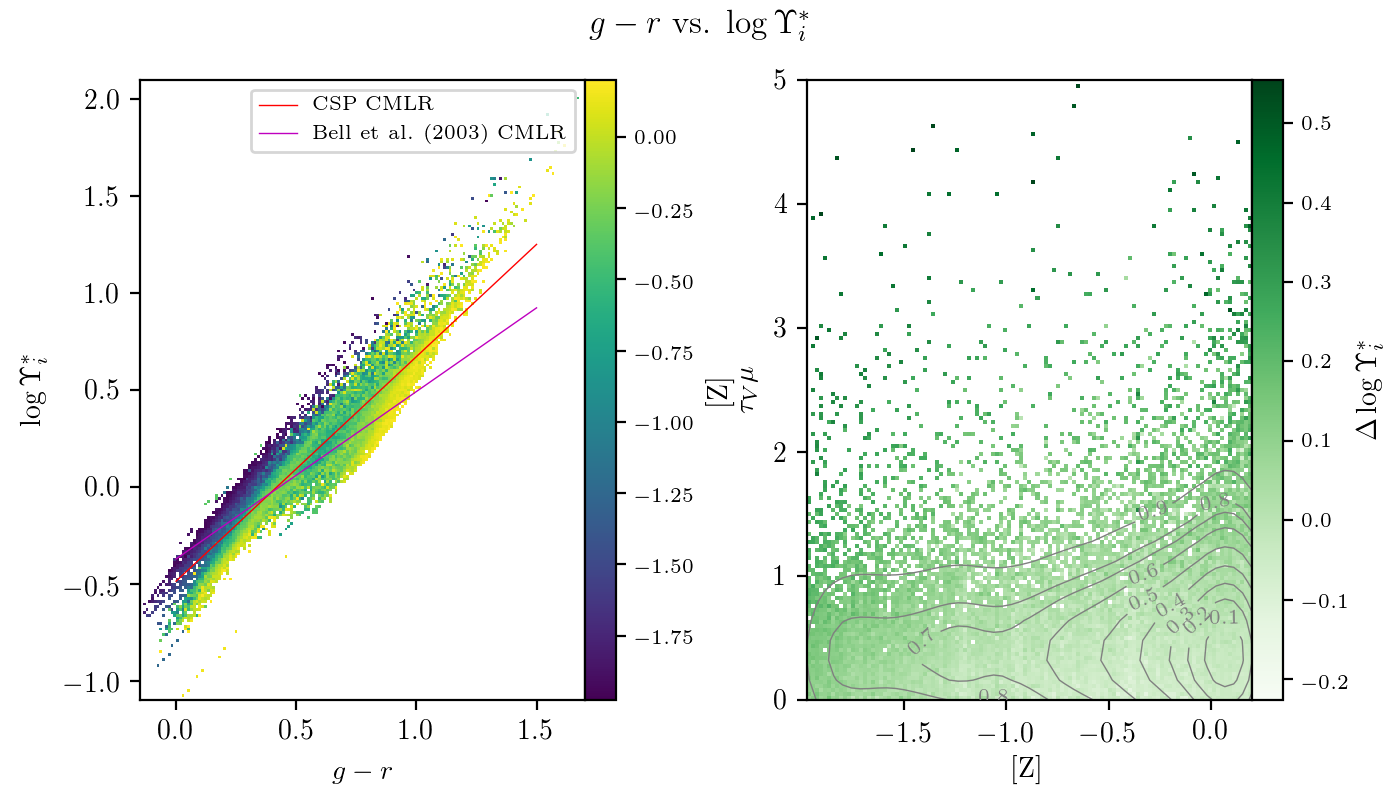
\includegraphics[width=\textwidth]{CMLRDiag_CgrMLi_logzsol-tau_V__mu-dev}
    \caption[Color--mass-to-light ratio relations ($g-r$ to $i$-band) for the training data]{\fixspacing Left-hand panel: effective $i$-band stellar mass-to-light ratios (in solar units) for model spectra generated  above, plotted against rest-frame $g-r$ color, and colored by stellar metallicity; in \emph{red}, the CMLR obtained from a least-squares fit to the CSP library; in \emph{magenta}, the CMLR from \citet{bell_03}, after a -0.15 dex Salpeter-to-Kroupa IMF correction. Right-hand panel: a visualization of the typical difference between a SFH's true stellar mass-to-light ratio and the mean CMLR at that color: each image pixel is colored according to the median of the CMLR deviation for all CSPs in that small ${\rm [Z]}$--$\tau_V \mu$ bin (or white, if there are none). Overlaid in red contours is shown the approximate fraction of models within a given contour (derived from a two-dimensional kernel density estimation).}
    \label{fig:CMLR_Cgr-MLi-dev}
\end{figure*}

\begin{figure*}
    \centering
    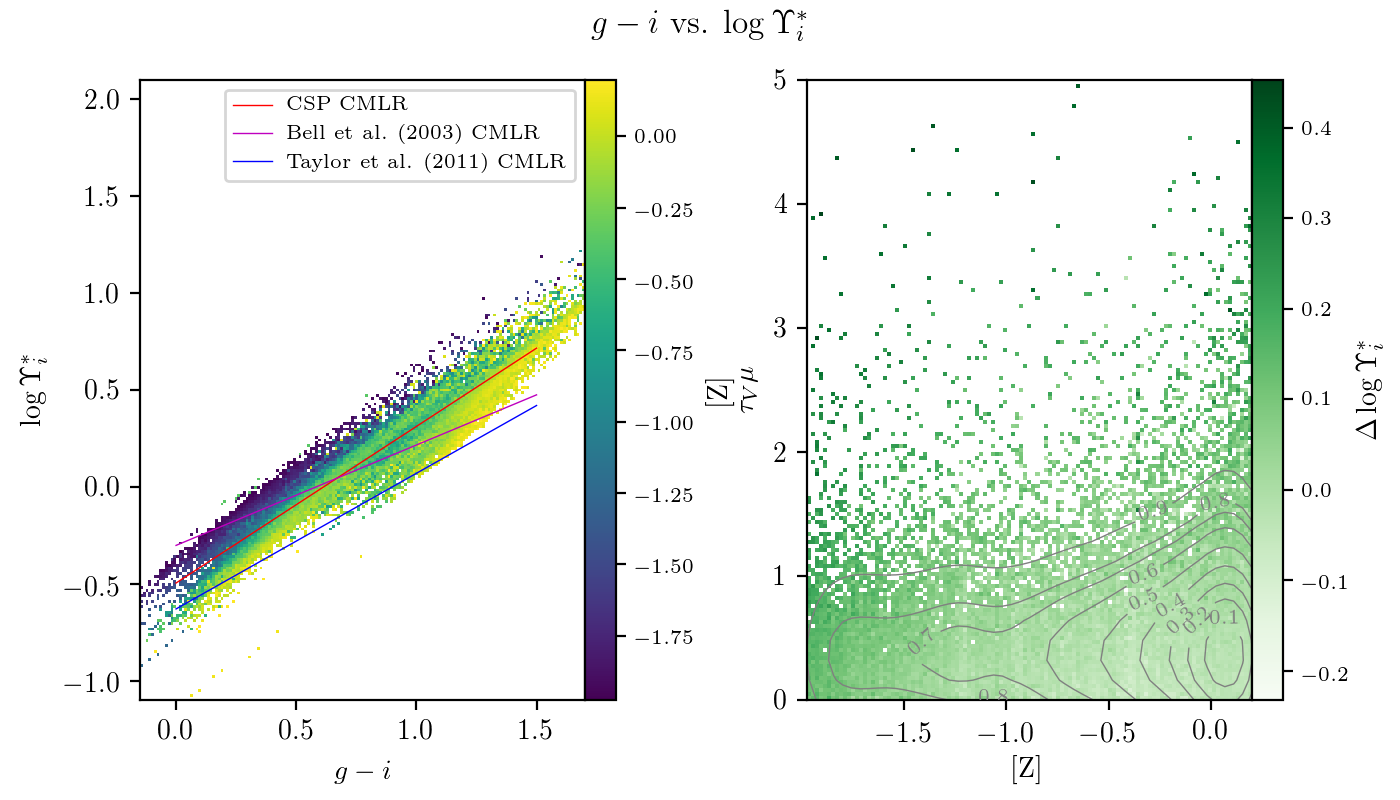
\includegraphics[width=\textwidth]{CMLRDiag_CgiMLi_logzsol-tau_V__mu-dev}
    \caption[Color--mass-to-light ratio relations ($g-i$ vs $i$-band) for the training data]{\fixspacing As Figure \ref{fig:CMLR_Cgr-MLi-dev}, except calibrating $\log \Upsilon^*_i$ against $g-i$ color, plus \citet{taylor_gama_cmlrs} CMLR in the left-hand panel in \emph{blue}. All mass normalizations are once again corrected to \citet{kroupa_imf_01} IMF.}
    \label{fig:CMLR_Cgi-MLi-dev}
\end{figure*}

Overall, one should note that the scatter about the CMLR is not entirely random. This means that even before systematics related to stellar model atmospheres and our fiducial SFH family, the functional lower-limit on stellar mass-to-light ratio uncertainty is about 0.1 dex. Especially in the case of vigorous recent star-formation, stellar metallicity is associated with pronounced departures from the ``mean" CMLR (the large number of blue, low-metallicity models at higher-than-predicted mass-to-light ratios is one noticeable example). Figures \ref{fig:CMLR_Cgr-MLi-dev} and \ref{fig:CMLR_Cgi-MLi-dev} show that while CSPs in the most common regions of parameter space have their stellar mass-to-light ratios described well by the best-fit CMLR, departures from the median case can cause troublesome systematics: for instance, at low metallicity, $\Delta \logml{i}$ can reach values of 0.2--0.3 dex, even at low attenuations; and higher optical depths ($\tau_V \mu \sim 3$) can boost this discrepancy as high as 0.4 dex. This is not simply a scatter about the CMLR, but is rather a true systematic. The effect is similar in ${\rm [Z]}-\tau_V (1 - \mu)$ space.

To illustrate the potential effects of attenuation in pulling a single SFH away from a CMLR, consider the following scenario: at fixed fractional optical depth $\mu = 0.4$, a SFH with $t_{form} = \tau = 2~{\rm Gyr}$ changes in $g-r$ color and $\log \Upsilon^*_i$ by +0.094 and +0.14 when $\tau_V$ is changed from 0.0 to 1.0, a considerably steeper slope than the fiducial CMLR. Furthermore, the slope of the attenuation vector in $(g-r)$--$\log \Upsilon^*_i$ space increases with $\mu$, matching the slope of the CMLR at $\mu \sim 0.14$ (recall that $\mu$ affects the balance between attenuation of young stars and old). In \citet{bell_dejong_01} and \citet{bell_03}, attenuation was explicitly ignored, because the attenuation vector lay almost parallel in color--mass-to-light space to the adopted CMLR. Depending on the exact value of $\mu$, this may not be true. So, for the SFH chosen above, the stellar mass-to-light ratio is under-estimated for most realistic values of $\mu$ and $\tau_V$.

Also a concern is the effect of the stellar IMF on the relative mass normalization. Using 1000 separately-randomized SFHs for three of the five stellar IMFs built into \texttt{FSPS}\footnote{It was computationally less costly to randomize each IMF's set of SFHs than it was to use the same SFHs using each of the three IMFs.}---\citet{salpeter_imf_55}, \citet{chabrier03}, and \citet{kroupa_imf_01}---, we have separately-determined the $\Upsilon^*_i$ normalization and its overall dependence on $g-r$ color (see Table \ref{tab:cmlr_fit}) for our training library. The effects of IMF on integrated colors are of course small (and likely attributable to differences in SFH randomization), but the overall mass normalizations differ quite strongly: \citet{kroupa_imf_01} and \citet{chabrier03} are offset respectively by $-0.209~{\rm dex}$ and $-0.252~{\rm dex}$, with respect to \citet{salpeter_imf_55}.

\begin{table}
    \centering
    \begin{tabular}{||c|c|c|c||} \hline
        IMF & $m$ & $b$ & $\sigma~{\rm [dex]}$ \\ \hline 
        \citet{salpeter_imf_55} & 1.145 & -0.286 & 9.38 $\times 10^{-2}$ \\ \hline 
        \citet{kroupa_imf_01} & 1.147 & -0.496 & 9.62 $\times 10^{-2}$ \\ \hline 
        \citet{chabrier03} & 1.155 & -0.538 & 9.44 $\times 10^{-2}$ \\ \hline
    \end{tabular}
    \caption[Color--mass-to-light ratio relation linear fits]{\fixspacing Linear fit relating $g-r$ color to $\log \Upsilon^*_i$, and the magnitude of the scatter about the best-fit line (all a little less than 0.1 dex).}
    \label{tab:cmlr_fit}
\end{table}

In summary, CMLRs do not capture the full range of information contained in a galaxy's SED; indeed, they can also be susceptible to degeneracies between age, metallicity, and attenuation. Specifically, even at infinite signal-to-noise, both CMLRs tested here suffer from intrinsic scatter above the 0.05 dex level in the very common stellar metallicity range of -0.5--0.2 and at diffuse ISM optical depths greater than 1.0. Deviations from a fiducial dust law can also induce changes in the effective stellar mass-to-light ratio which are \emph{not} parallel to the CMLR, as had been previously suggested \citep{bell_dejong_01, bell_03}. There is much more information to glean from galaxy SEDs than can be encoded in optical colors.
